\chapter{Autoencoder}
% Authors: Chengze Zuo 2019-04-11
    
The following code shows some example codes of the basic class structure for autoencoders and some experiments for the autoencoder (under-complete) and the denoising autoencoder (over-complete)
\section{Some preparation step for img vector processing and the display method}
\begin{minted}{python}
def to_img(x):
    x = 0.5 * (x + 1)
    x = x.view(x.size(0), 28, 28)
    return x       
\end{minted}
        
\begin{minted}{python}
# Displaying routine

def display_images(in_, out, n=1):
    for N in range(n):
        if in_ is not None:
            in_pic = to_img(in_.cpu().data)
            plt.figure(figsize=(18, 6))
            for i in range(4):
                plt.subplot(1,4,i+1)
                plt.imshow(in_pic[i+4*N])
                plt.axis('off')
        out_pic = to_img(out.cpu().data)
        plt.figure(figsize=(18, 6))
        for i in range(4):
            plt.subplot(1,4,i+1)
            plt.imshow(out_pic[i+4*N])
            plt.axis('off')    
\end{minted}

\section{Define model architecture, reconstruction loss and configure the optimizer}

Each image in MNIST has dimension of 28 x 28. The dimension for hidden layer could be set to 30 (for under-complete) and 500 (for over-complete)

\begin{minted}{python}
# Define model architecture and reconstruction loss

# n = 28 * 28 # 784
d = 30  # for standard AE (under-complete hidden layer)
# d = 500  # for denoising AE (over-complete hidden layer)

class Autoencoder(nn.Module):
    def __init__(self):
        super().__init__()
        self.encoder = nn.Sequential(
            nn.Linear(28 * 28, d),
            nn.Tanh(),
        )
        self.decoder = nn.Sequential(
            nn.Linear(d, 28 * 28),
            nn.Tanh(),
        )

    def forward(self, x):
        x = self.encoder(x)
        x = self.decoder(x)
        return x
    
model = Autoencoder().to(device)
criterion = nn.MSELoss()
\end{minted}

\begin{minted}{python}
# Configure the optimiser

learning_rate = 1e-3

optimizer = torch.optim.Adam(
    model.parameters(),
    lr=learning_rate,
)
\end{minted}

\section{Training the autoencoder, denoising autoencoder, and check on the learned kernel}
\begin{minted}{python}
# Train standard or denoising autoencoder (AE)

num_epochs = 3
# do = nn.Dropout()  # comment out for standard AE
for epoch in range(num_epochs):
    for data in dataloader:
        img, _ = data
        img = img.to(device)
        img.requires_grad_()
        img = img.view(img.size(0), -1)
#         img_bad = do(img).to(device)  # comment out for standard AE
        # ===================forward=====================
        output = model(img)  # feed <img> (for std AE) or <img_bad> (for denoising AE)
        loss = criterion(output, img.data)
        # ===================backward====================
        optimizer.zero_grad()
        loss.backward()
        optimizer.step()
    # ===================log========================
    print(f'epoch [{epoch + 1}/{num_epochs}], loss:{loss.item():.4f}')
    display_images(None, output)  # pass (None, output) for std AE, (img_bad, output) for denoising AE
    
display_images(None, model.encoder[0].weight, 5)
\end{minted}

For training the under-complete autoencoder, in the code we comment out the \textbf{img\_bad}, the dropout and just pass the \textbf{img} as the argument into the model. While training the denoising autoencoder, we we uncomment the \textbf{img\_bad}, activate the dropout (because it will deactivate some neurons and add "noise" to the network) and pass the \textbf{img\_bad} it (instead of \textbf{img}) to the model. After executing the \textbf{display\_images}, we could visualize the learned kernels.

For under-complete autoencoders (d = 30), the decoding images are shown:

\begin{figure}[htb]
    \centering
    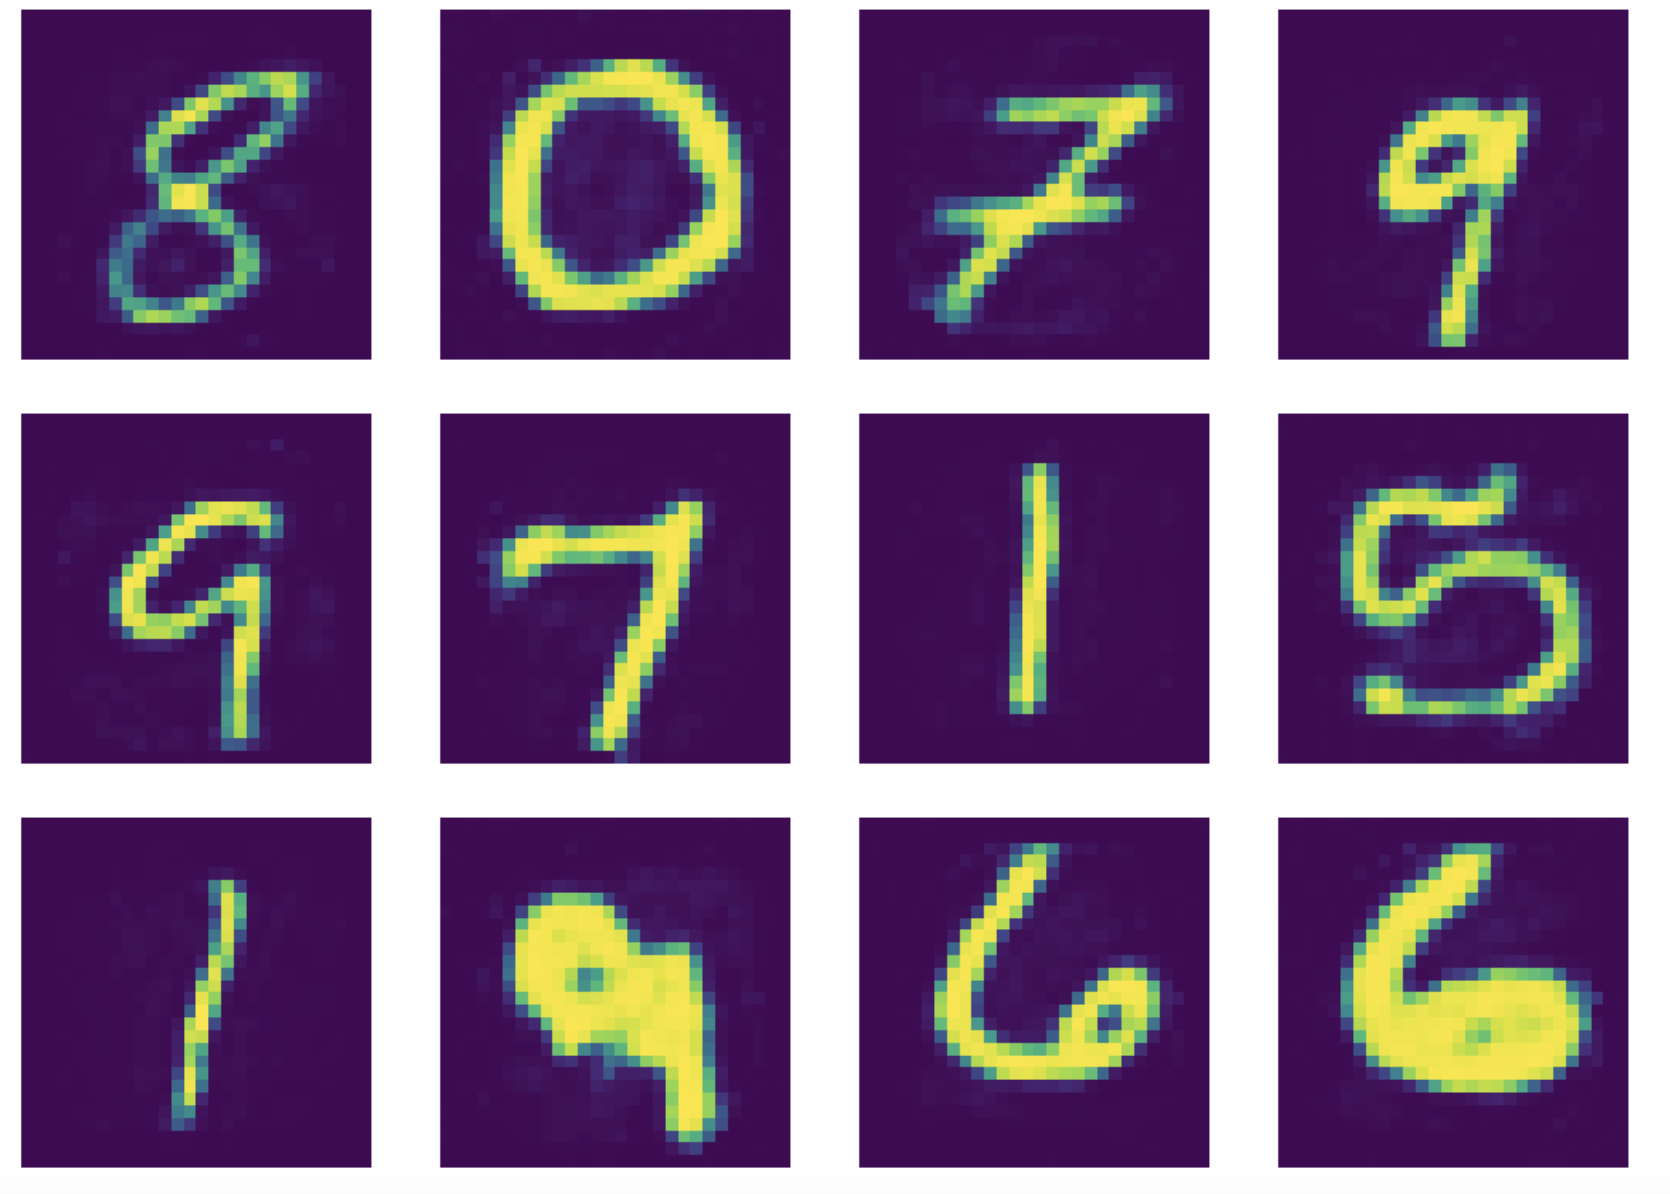
\includegraphics[width=0.6\textwidth]{labs/10/images/Autoencoder.png}
    \caption{Reconstructed images by the autoencoder}
    \label{fig:Autoencoder}
\end{figure}

The learned kernels for the first layer are shown:

\begin{figure}[htb]
    \centering
    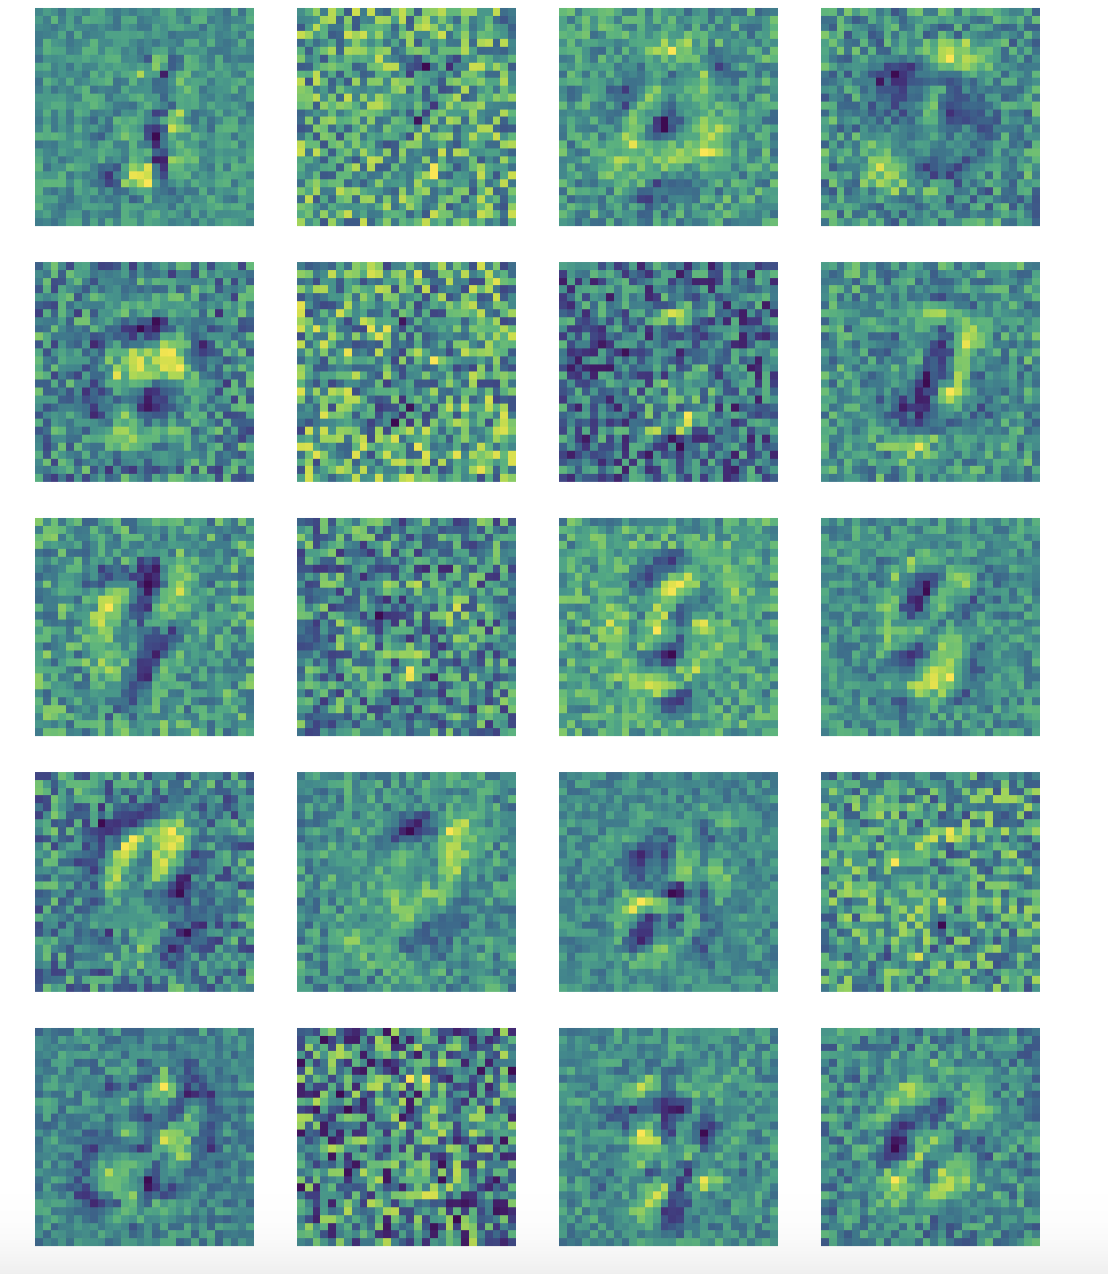
\includegraphics[width=0.6\textwidth]{labs/10/images/AE_kernels.png}
    \caption{Learned kernels for the autoencoder (d=30)}
    \label{fig:AE kernels}
\end{figure}

For denoising autoencoders (d = 500), the decoding images are shown:

\begin{figure}[H]
    \centering
    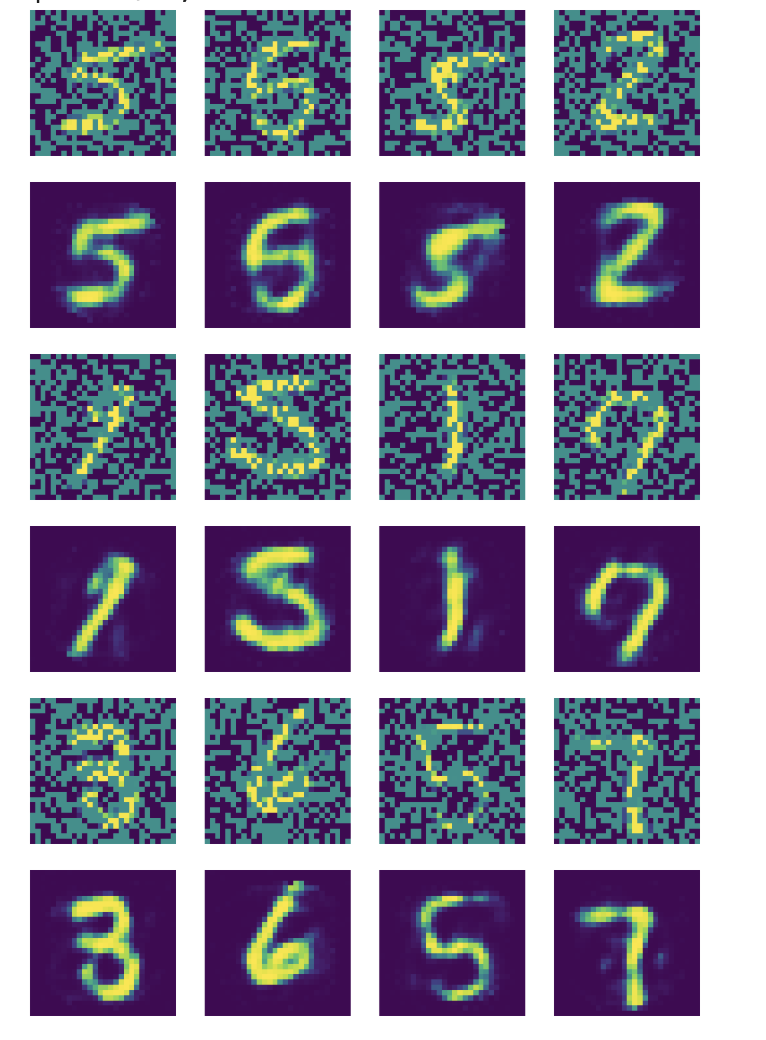
\includegraphics[width=0.6\textwidth]{labs/10/images/Denoising_AE.png}
    \caption{Reconstructed images by the denoising autoencoder}
    \label{fig:Denosing Autoencoder}
\end{figure}

As shown from the picture, the denosing AE perform much better than the under-complete AE in terms of image reconstruction, especially a some specific images.

The learned kernels for the first layer are shown: 

\begin{figure}[H]
    \centering
    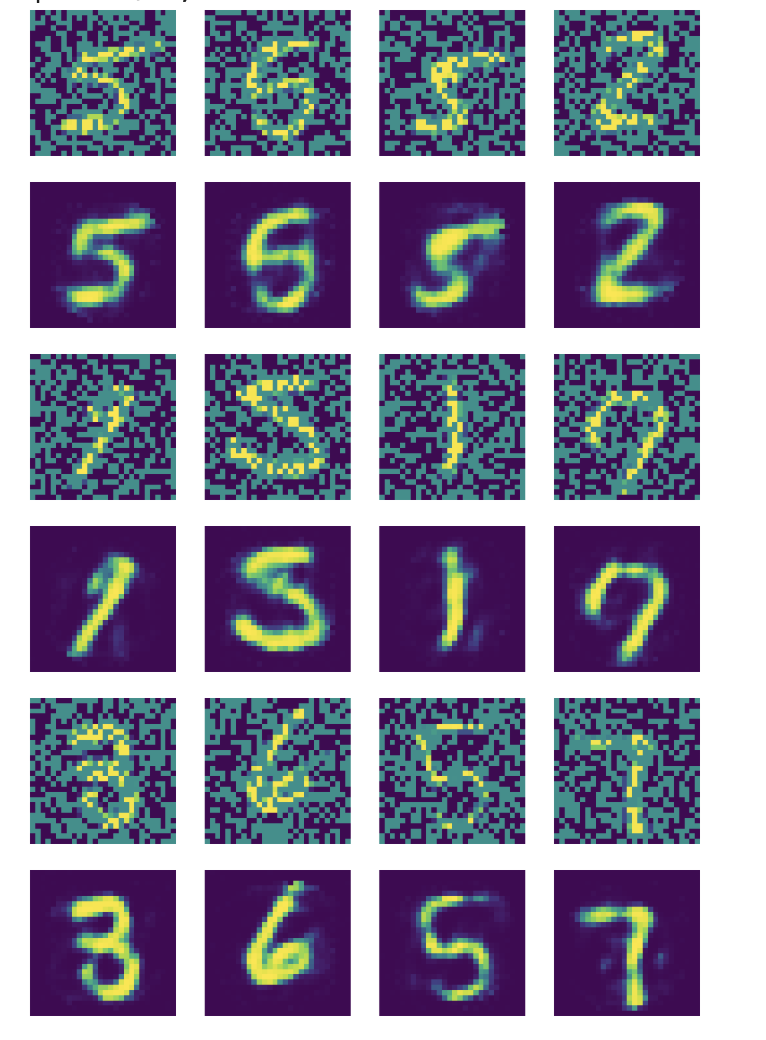
\includegraphics[width=0.6\textwidth]{labs/10/images/Denoising_AE.png}
    \caption{Reconstructed images by the denoising autoencoder}
    \label{fig:Denoising AE kernels}
\end{figure}

where some of the kernels learned from the denoising AE have much more clearer "edges" compared to the kernels learned from the under-complete AE. Note that some kernels are really "noisy" because of the randomness introduced by dropout, cause some neurons and weights are shut down and unlearned.

\section{Inpaint comparison with Telea and Navier-Stokes methods}

\begin{minted}{python}
# Let's compare the autoencoder inpainting capabilities vs. OpenCV

from cv2 import inpaint, INPAINT_NS, INPAINT_TELEA

# Inpaint with Telea and Navier-Stokes methods

dst_TELEA = list()
dst_NS = list()

for i in range(3, 7):
    corrupted_img = ((img_bad.data.cpu()[i].view(28, 28) / 4 + 0.5) * 255).byte().numpy()
    mask = 2 - img_bad.grad_fn.noise.cpu()[i].view(28, 28).byte().numpy()
    dst_TELEA.append(inpaint(corrupted_img, mask, 3, INPAINT_TELEA))
    dst_NS.append(inpaint(corrupted_img, mask, 3, INPAINT_NS))

tns_TELEA = [torch.from_numpy(d) for d in dst_TELEA]
tns_NS = [torch.from_numpy(d) for d in dst_NS]

TELEA = torch.stack(tns_TELEA).float()
NS = torch.stack(tns_NS).float()

# Compare the results: [noise], [img + noise], [img], [AE, Telea, Navier-Stokes] inpainting

with torch.no_grad():
    display_images(img_bad.grad_fn.noise[3:7], img_bad[3:7])
    display_images(img[3:7], output[3:7])
    display_images(TELEA, NS)
\end{minted}

The main point for last part is to achieve better model performance, you had better make the network learn from the data, which Navier-Stokes and Telea approaches did not do that.